\RequirePackage{luatex85}
\documentclass[eqno]{ltjsarticle}
\usepackage{luatexja-fontspec}
\usepackage[a4paper, top=25mm, bottom=25mm, left=25mm, right=25mm]{geometry}
\usepackage{luatexja} 
\usepackage{multicol,amsmath,amssymb,mathtools,ascmac,amsthm,amscd,physics,comment,dcolumn,titlesec,mathrsfs,test,tikz-cd,enumitem}
\usetikzlibrary{arrows.meta,calc}
\titleformat*{\section}{\Large\bfseries}
\setlength{\parindent}{0pt}
\usepackage[most]{tcolorbox}
\tikzset{every picture/.style={remember picture,baseline=(current bounding box.center)}}
%\everymath{\displaystyle}
\begin{document}
\title{安定性条件}
\date{}
\author{大阪大学大学院理学研究科数学専攻\\山本 雄大}
\maketitle
\tableofcontents
\section{三角圏の公理}
\begin{defn}
	圏$\C$が前加法圏(preadditive category)とは,以下を満たす場合である.
	\vspace{-3mm}
	\begin{itemize}
		\item[(i)]
			任意の$E,F\in\C$に対して,$\Hom_{\C}(E,F)$がAbel群になる.
		\item[(ii)]
			任意の$E,F,G\in\C$に対して,
		\[
			\begin{array}{ccccc}
				\Hom_{\C}(F,G) \times \Hom_{\C}(E,F) & \longrightarrow & \Hom_{\C}(E,G) \\
				\rotatebox{90}{\in}& &\rotatebox{90}{\in}\\
															(g, f) & \longmapsto & g \circ f
					\end{array}
\]
が双線型である.つまり,任意の$g,g'\in\Hom_{\C}(F,G),\ f,f'\in\Hom_{\C}(E,F)$に対して,
\begin{gather}
	(g+g')\circ f = g\circ f + g'\circ f\\
	g\circ(f+f') = g\circ f + g\circ f'
\end{gather}
	\end{itemize}
\end{defn}
が成り立つ.

\begin{defn}
	前加法圏$\C$が加法圏(additive category)であるとは,
	\vspace{-3mm}
	\begin{itemize}
	\item[(i)]零対象(始対象かつ終対象)である$0\in\C$をを持つ.
	\item[(ii)]任意の対象$E,F\in\C$に対し直和$E\oplus F$が存在する.
	\end{itemize}
	\vspace{-3mm}
\end{defn}

\begin{defn}
	加法圏$\D$がアーベル圏であるとは
\end{defn}

\begin{defn}
	$\D$を加法圏,$[1]$を自己同値函手とする.
	完全三角形と呼ばれる$\D$における三角形の集合を備えた,以下の性質をみたす組$(\D,[1])$を三角圏と呼ぶ$$$$
	\vspace{-3mm}
	\begin{itemize}
		\item[(i)]
			任意の$E\in\D$に対して,
			\[E\xrightarrow{\id_E}E\rightarrow 0 \rightarrow E[1]\]
			は完全三角形.
		\item[(ii)]
			\[
		\begin{tikzcd}
			E_1\ar[r]\ar[d,"f"]& E_2\ar[r]\ar[d,"g"]& E_3\ar[r]\ar[d,"h"] & E_1[1]\ar[d,"f\texttt{[1]}"]\\
			F_1\ar[r]& F_2\ar[r]& F_3\ar[r] & F_1[1]\\
		\end{tikzcd}
			\]
			上の可換図式において,$f,g,h$が同型で$E_1\rightarrow E_2\rightarrow E_3 \rightarrow E_1[1]$が完全三角形なら$F_1\rightarrow F_2\rightarrow F_3 \rightarrow F_1[1]$も完全三角形
		\item[(iii)]
			任意の$E\xrightarrow{f}F$は
			\[E\xrightarrow{f} F\rightarrow G \rightarrow E[1]\]
		と完全三角形に拡張できる.
	\item[(iv)]
		\[
			E_1\xrightarrow{u} E_2\xrightarrow{v} E_3\xrightarrow{w}  E_1[1]
	\]
	が完全三角形であることと
	\[
		E_2\xrightarrow{v} E_3\xrightarrow{w} E_1\xrightarrow{-u[1]}  E_2[1]
	\]
	が完全三角形であることが同値.
	\item[(v)]
		\[
		\begin{tikzcd}
			E_1\ar[r]\ar[d,"f"]& E_2\ar[r]\ar[d,"g"]& E_3\ar[r]\ar[d,"h",dotted] & E_1[1]\ar[d,"f\texttt{[1]}"]\\
			F_1\ar[r]& F_2\ar[r]& F_3\ar[r] & F_1[1]\\
		\end{tikzcd}
	\]
	2つの完全三角形と図式を可換にする$f,g$が存在したとき,すべての四角形を可換にする$h$が存在する.

	\item[(vi)]
		八面体公理\\
			\[
				\begin{tikzcd}[row sep=5pt]
			E \ar[r,"f"]& F\ar[r,"h"]& X \ar[r]& E[1]\\
			E \ar[r,"g\circ f"]& G\ar[r,"l"]& Y \ar[r]& E[1]\\
			F \ar[r,"g"]& G\ar[r,"k"]& Z \ar[r]& F[1]\\
		\end{tikzcd}
			\]
			上記の3つの完全三角形に対して,以下の図式のすべての四角形を可換にし,4行目を完全三角形にするような$u\in\Hom_{\D}(X,Y),v\in\Hom_{\D}(Y,Z),w\in\Hom_{\D}(Z,X[1])$が存在する.
			\[
		\begin{tikzcd}
			E \ar[r,"f"]\ar[d,equal]& F\ar[r,"h"]\ar[d,"g",swap]& X\ar[d,"u",dotted] \ar[r]& E[1]\ar[d,equal]\\
			E \ar[r,"g\circ f"]\ar[d,"f",swap]& G\ar[r,"l"]\ar[d,equal]& Y\ar[d,"v",dotted] \ar[r]& E[1]\ar[d,"f\texttt{[1]}"]\\
			F \ar[r,"g"]\ar[d,"h",swap]& G\ar[r,"k"]\ar[d,"l",swap]& Z \ar[r]\ar[d,equal]& F[1]\ar[d,"h\texttt{[1]}"]\\
			X \ar[r,"u",dotted]& Y\ar[r,"v",dotted]& Z \ar[r,"w",dotted]& X[1]\\
		\end{tikzcd}
			\]
	\end{itemize}
\end{defn}

\section{t-structure}
\begin{defn}\cite{BBD}
		$\D$を三角圏.直和因子と同型を取る操作で閉じている加法部分圏$\D^{\le 0},\D^{\ge 0}\subset\D$が次の条件を満たすとき,$(\D^{\le 0},\D^{\ge 0})$を$\D$のt-構造と呼ぶ.
		$\D^{\le n}\coloneq\D^{\le 0}[-n],\hspace{3mm}\D^{\ge n}\coloneq\D^{\ge 0}[-n] $
		\begin{itemize}
			\item[(i)]
				$\D^{\le 0}\subset\D^{\le 1}\hspace{3mm}\D^{\ge 1}\subset\D^{\ge 0} $
			\item[(ii)]
				$\D^{\ge 1}\subset (\D^{\le 0})^\perp$\\
				つまり,$\forall E\in \D^{\le 0},\ \forall F\in\D^{\ge 1},\ \Hom_{\D}(E,F)=0$
			\item[(iii)]
				任意の$E\in\D$に対して
				\[\tau_{\le 0}E\rightarrow E \rightarrow \tau_{\ge 1}E\rightarrow \tau_{\le 0}E[1]\]
				となるような$\tau_{\le 0}E\in\D^{\le 0},\ \tau_{\ge 1}E\in\D^{\ge 1}$が存在する.
		\end{itemize}
\end{defn}

\begin{lemm}
		\begin{itemize}
				\item[(i)]$\D^{\ge 1}=(\D^{\le 0})^{\perp}$
				\item[(ii)]$E\in\D$に対して,$\tau_{\le 0}E\in\D^{\le 0}, \tau_{\ge 1}E\in\D^{\ge 1}$は同型を除いて一意に定まる.
		\end{itemize}
\end{lemm}
	\begin{proof}
		$E\in\mathcal (\D^{\le 0})^\perp$ を任意にとる.定義より以下の完全三角形がとれる.
				\[\tau_{\le 0}E\rightarrow E \rightarrow \tau_{\ge 1}E\rightarrow \tau_{\le 0}E[1]\]
				定義より,$\tau_{\le 0}E\rightarrow E$は0射であるので,$\tau_{\ge 1}E\simeq E\oplus\tau_{\le 0}E[1]\in \D^{\ge 1}$.直和因子と同型を取る操作で閉じているので$E\in\D^{\ge 1}$.\\
				一意性については,別の$F\in\D^{\le 0},\ G\in\D^{\ge 1}$と完全三角形
				\[F\rightarrow E \rightarrow G\rightarrow F[1]\]
\end{proof}
\begin{defn}\cite{BBD}
	$(D^{\le 0},\D^{\ge 0})$がt-構造を与えるとき,$\D$の部分圏$\H\coloneq\D^{\le 0}\cap\D^{\ge 0}$はt-構造の核(the heart of t-structure)と呼ばれる.
\end{defn}

\begin{lemm}\cite{BBD}
	$\H$は核,余核をもつ.
\end{lemm}
\begin{proof}
	$E,F\in\H$,$f\in\Hom_{\H}(E,F)$を任意にとる.このとき,三角圏の公理より以下の完全三角形
	\[C\xrightarrow{e}A\xrightarrow{f}B\xrightarrow{g}C[1]\]
	が存在する.t-構造の定義より
	\[X\xrightarrow{x}C[1]\xrightarrow{y}Y\rightarrow X[1]\]
	が完全三角形となるような$X\in \D^{\le -1},Y\in \D^{\ge 0}$が存在する.このとき,
	\[y\circ g\colon B\rightarrow Y\]
	が$f$の余核を与えることを示す.
	\begin{comment}
			\[
				\begin{tikzcd}[column sep=huge,row sep =huge]
					B[-1] \ar[r,"g\texttt{[-1]}"]\ar[d,equal]& C\ar[r,]\ar[d,"y\texttt{[-1]}",swap]& A\ar[d,"\ell",dotted] \ar[r,"f"]& B\ar[d,equal]\\
					B[-1] \ar[r,"y\texttt{[-1]}\circ g\texttt{[-1]}"]\ar[d,"g\texttt{[-1]}",swap]& Y[-1]\ar[r,]\ar[d,equal]& M\ar[d,dotted] \ar[r,"m"]& B\ar[d,"g"]\\
					C \ar[r,]\ar[d,swap]& Y[-1]\ar[r,]\ar[d,swap]& X \ar[r,"x"]\ar[d,equal]& C[1] \ar[d,]\\
			A \ar[r,"\ell",dotted]& M\ar[r,dotted]&  X\ar[r,dotted]& A[1]\\
		\end{tikzcd}
			\]
\end{comment}	
			定義より,$A\in\H\subset\D^{\le 0}$,$X\in\D^{\le -1}\subset\D^{\le 0}$であり,八面体公理より存在する以下の完全三角形から
	\[A\rightarrow M\rightarrow X\rightarrow A[1]\]
	$M\in\D^{\le 0}$がわかる.$B\in\H\subset\D^{\le 0}$,$A[1]\in \D^{\le -1}\subset \D^{\le 0}$より$C[1]\in\D^{\le 0}$がしたがう.$X[1]\in\D^{\le -2}\subset\D^{\le 0}$と合わせて,$Y\in\D^{\le 0}$がしたがう.取り方により$Y\in\D^{\ge 0}$だったので$Y\in\H$がわかる.\\
	$Q\in\H$と$q\circ f$を満たす$q\in\Hom_{\H}(B,Q)$を任意にとると,$q=q'\circ g$を満たす$q'\in\Hom_{\D}(C[1],Q)$が存在する.また,$X\in\D^{\le -1}$,$Q\in\D^{\ge 0}$なので$g\circ q'=0$.したがって,$q'=y\circ q''$を満たす$q''\in\Hom_{\D}(Y,Q)$が存在する.完全系列
	\[A\rightarrow B\xrightarrow{g} C[1]\rightarrow A[1]\]
	に対して,コホモロジー的函手$\Hom_{\D}(-,Q)$を作用させると$A[1]\in\D^{\le -1}$なので$\Hom_{\D}(A[1],Q)=0$から完全列
	\[0\rightarrow \Hom_{\D}(C[1],Q) \rightarrow \Hom_{\D}(B,Q)\]
	が存在して,$q=q'\circ g$となる$q'$の一意性がわかる.どうように$X[1]\in\D^{\le -1}$なので,
	\[0\rightarrow \Hom_{\D}(Y[1],Q) \rightarrow \Hom_{\D}(C[1],Q)\]
	$q'=q''\circ y$となる$q''$の一意性がわかる.したがって,$y\circ g\colon B\to Y$が$f\colon Ato B$の余核を与えていることが示された.反対圏を考えることで核の存在も証明される.
\end{proof}

\begin{thm}
	$\H$はアーベル圏となる.
\end{thm}
\begin{proof}
	核,余核の存在は示されたので任意の射$f\in\Hom_{\H}(A,B)$にたいして,
\[\Im(f)\simeq \Coim(f)\]
の存在を言えばよい.
\end{proof}

\begin{lemm}
	$\D$を三角圏,$\A\subset\D$を充満部分加法圏としたとき,$\A$有界なt-構造$\F\subset\D$の核であることと以下の条件が同値.\vspace{-3mm}
	\begin{enumerate}[label=\roman*.]
		\item
			任意の$k_1,k_2\in\ZZ\ (k_1>k_2)$と$A,B\in\A$に対して,$\Hom_{\D}(A[k_1],B[k_2])=0$
		\item
			任意の対象$E\in\D$に対して,有限の整数の列
			\[k_1>k_2 \cdots > k_n\]
			が存在して$A_j\in \A[k_j]$となるような分解が存在する.
	\end{enumerate}
\end{lemm}
\begin{proof}
	\[
		\begin{tikzcd}[column sep=1.3em]
			0\ar[r,equal]&E_0\ar[rr]& & E_{1}\ar[r]\ar[ld] &\cdots\ar[r] &E_{n-2}\ar[rr]&&E_{n-1}\ar[ld]\ar[rr]&&E_n\ar[ld]\ar[r,equal]&E\\
									 &&A_{1}\ar[lu,dotted,"{[1]}"] &&&&A_{n-1}\ar[lu,dotted,"{[1]}"]&&A_n\ar[lu,dotted,"{[1]}"]
		\end{tikzcd}
	\]
				
	\end{proof}

\section{安定性条件}
	

\begin{defn}\cite{Bristab}
		アーベル圏$\A$上の安定性条件とは群準同型
		\[Z\colon K(\A)\to \CC\]
		で以下を満たすもの
\begin{itemize}
	\item[(i)]
		$\forall E(\neq 0)\in\A, Z(E)\in\HH\coloneq \{re^{i\pi\phi}\mid r>0, 0<\phi \le 1\}$
	\item[(ii)]
		任意の$E\in\A$に対してHNフィルトレーションが存在する.
		\[0=E_0\subset E_1\subset \cdots \subset E_k = E\]
		で各$F_i = E_i/E_{i-1}$が$Z$について$Z$-半安定.
\end{itemize}
$E(\neq 0)$が$Z$-半安定とは任意の部分対象$0\neq F\subsetneq E$に対して,$\arg Z(F) \le \arg Z(E)$
ここで,
\[\phi(E)\coloneq \frac{1}{\pi}\arg Z(E)\in (0,1] \]
と定める.
\end{defn}	

\begin{lemm}
	$E,F\in\D$が半安定で$\phi(E)>\phi(F)$とき,
	\[\Hom_{\D}(E,F)=0\]
\end{lemm}
\begin{pf}
	$f\in\Hom_{\D}(E,F)$が$0$でないと仮定する.
	\[0\rightarrow\Ker f\rightarrow E \rightarrow \Im f \rightarrow 0\]
	の完全列が存在して$E$が半安定対象であることから$\phi(\Im f)\ge\phi(E)$.$\Im f\neq 0$が$F$の部分対象で$F$も半安定であることから$\phi(F)\ge\phi(\Im f)$.これらを合わせると$\phi(F)\ge\phi(E)$.仮定に矛盾.
\end{pf}

\begin{lemm}\cite{Bristab}
		$\A\colon$アーベル圏,群準同型$Z\colon K(\A)\to \CC$が次の条件を満たすとき,HNフィルトレーションが存在する.つまり$Z$が安定性条件を定める.
		\begin{itemize}
			\item[(i)]
			全射の無限列
		\[E_1\twoheadrightarrow E_2\twoheadrightarrow E_3\twoheadrightarrow\cdots  \]
		で$\phi (E_i)> \phi (E_{i+1})$となるものは存在しない.
	\item[(ii)]
			無限降下列
		\[E_1\supset E_2\supset E_3\supset \cdots  \]
		で$\phi (E_{i+1}) > \phi(E_i)$となるものは存在しない.
	\end{itemize}
\end{lemm}

\begin{proof}\hfil
	\begin{screen}
	Step 1\hspace{5mm}\\
	\bullet 任意の対象$E\in\A$には$\phi(A) \ge \phi(E)$を満たす半安定な部分対象$A$が存在する.\\
	\bullet 任意の対象$E\in\A$には$\phi(E) \ge \phi(B)$を満たす半安定な対象$B$と全射$E\twoheadrightarrow B$が存在する.
\end{screen}
	$E$が半安定ならOK.そうでないなら$\phi(E')>\phi(E)$となる部分対象$E'(\subsetneq E)$がとれる.\\
	これが無限回繰り返されると条件の(ii)に矛盾するので有限回でとまる.この極小となる$A$をとれば半安定である.\\
	同様に$E$が半安定なら全射$E\xrightarrow{\id}E$がとれてOK.そうでないとき,$E'(\subsetneq E)$で,$\phi(E')>\phi(E)$が存在して,$B'\coloneq E/E'$と定めると$\phi(E)\ge\phi(B')$であり,$E\twoheadrightarrow E/E'$がとれて,有限回でこの操作はとまるのでいずれ半安定になる.
\begin{center}
	\usetikzlibrary{arrows.meta}

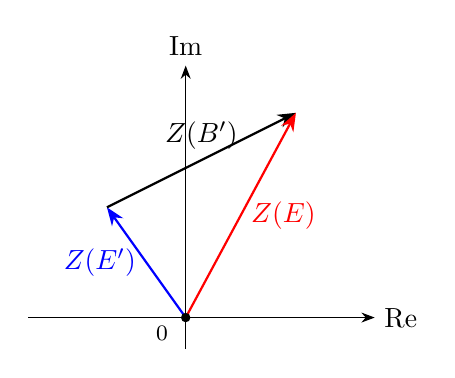
\begin{tikzpicture}[scale=2, >=Stealth]

  % 原点を中心に設定
  \coordinate (O) at (0,0);

  % 各ベクトルの終点
  \coordinate (E') at (-0.5,0.7);     % Z(A)
  \coordinate (B') at (1.2,0.6);    % Z(E/A)
  \coordinate (E) at ($(E')+(B')$); % Z(E) = Z(A) + Z(E/A)

  % 軸
  \draw[->] (-1,0) -- (1.2,0) node[right] {\(\Re\)};
  \draw[->] (0,-0.2) -- (0,1.6) node[above] {\(\Im\)};

  % Z(A) ベクトル(青)
  \draw[->, thick,blue] (O) -- (E') node[midway, left] {\(Z(E')\)};

  % Z(E/A) ベクトル(緑):Aの先から
  \draw[->, thick] (E') -- (E) node[midway,above] {\(Z(B')\)};

  % Z(E) ベクトル(赤):原点から
  \draw[->, thick,red] (O) -- (E) node[midway, right] {\(Z(E)\)};

  % 原点
  \fill (O) circle (0.03);
  \node at (-0.15, -0.1) {\footnotesize 0};

\end{tikzpicture}
\end{center}

	\begin{screen}
		Step 2\\
			$E\twoheadrightarrow B$が次の条件をみたすときmdqと呼ぶ.\\
			\bullet $\phi(E)\ge\phi(B)$\\
			\bullet 任意の$E\twoheadrightarrow B'$に対して,$\phi(B')\ge \phi(B)$であり,$\phi(B')=\phi(B)$なら
			\[E\twoheadrightarrow B\twoheadrightarrow B'\]
			と分解.\\
			任意の対象$E$はmdqを持つ.
	\end{screen}
	$E\twoheadrightarrow B'$において$B'$が半安定でないならStep 1から半安定な対象$B''$で$\phi(B')>\phi(B'')$と$B'\twoheadrightarrow B''$がとれるので,$B'$が半安定なときについて示せばよい.同様にmdqの$B$は半安定でなければならない.\\
$E$が半安定対象のとき,任意の全射$E\twoheadrightarrow B'$に対して,短完全列
\[0\rightarrow \Ker f\rightarrow E\xrightarrow{f} B'\rightarrow 0\]
が存在するので$Z(B') = Z(E) - Z(\Ker f)$.安定対象なので,$\phi(\Ker f)\le \phi(E)$
\begin{center}
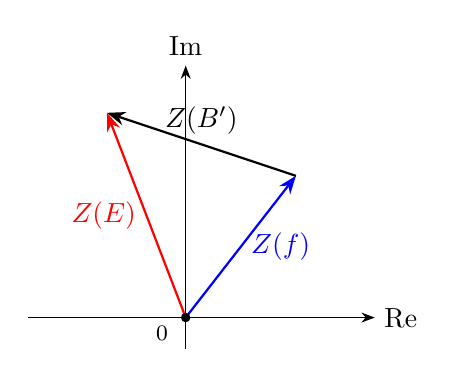
\begin{tikzpicture}[scale=2, >=Stealth]

  % 原点を中心に設定
  \coordinate (O) at (0,0);

  % 各ベクトルの終点
  \coordinate (Ker) at (0.7,0.9);     % Z(A)
  \coordinate (B') at (-1.2,0.4);    % Z(E/A)
  \coordinate (E) at ($(Ker)+(B')$); % Z(E) = Z(A) + Z(E/A)

  % 軸
  \draw[->] (-1,0) -- (1.2,0) node[right] {\(\Re\)};
  \draw[->] (0,-0.2) -- (0,1.6) node[above] {\(\Im\)};

  % Z(A) ベクトル(青)
  \draw[->, thick,blue] (O) -- (Ker) node[midway, right] {\(Z(\Ker f)\)};

  % Z(E/A) ベクトル(緑):Aの先から
  \draw[->, thick] (Ker) -- (E) node[midway,above] {\(Z(B')\)};

  % Z(E) ベクトル(赤):原点から
  \draw[->, thick,red] (O) -- (E) node[midway, left] {\(Z(E)\)};

  % 原点
  \fill (O) circle (0.03);
  \node at (-0.15, -0.1) {\footnotesize 0};

\end{tikzpicture}
\end{center}
したがって,$\phi(B')\ge\phi(E)$となり$E$が半安定対象のとき,$E\xrightarrow{\id}E$はmdqとなる.\\
そうでないとき,step1より$\phi(A)>\phi(E)$なる半安定対象$A\subsetneq E$と
\[0\rightarrow A\rightarrow E\rightarrow E'\rightarrow 0\]
という完全列が存在する.$\phi(A)>\phi(E)>\phi(E')$となっている.$E'\twoheadrightarrow B$が$E'$のmdqとなっているとき,合成$E\twoheadrightarrow B$は$E$のmdqであることを示す.\\
\because $E\twoheadrightarrow B'$を半安定で$\phi(B')\le \phi(B)$となっているとすると
\[\phi(A)>\phi(E)>\phi(E')\ge\phi(B)\ge\phi(B')\]
$A,B'$は半安定対象であり,前の補題より$\Hom_{\D}(A,B')=0$
\[\begin{tikzcd}
	A \ar[r,hookrightarrow]\ar[rd,"0",swap,]& E\ar[r,twoheadrightarrow]\ar[d,twoheadrightarrow]& E/A = E'\ar[ld,dotted,two heads]\\
								 &B'
\end{tikzcd}\]
図式のように可換にする全射が普遍性から存在する.$E'\twoheadrightarrow B$がmdqなので$\mu(B')=\mu(B)$となり,mdqの条件より$E'\twoheadrightarrow B\twoheadrightarrow B'$と経由する.したがって$E\twoheadrightarrow B\twoheadrightarrow B'$が存在し,$E\twoheadrightarrow B$がmdqであることがわかる.\\
$E'$がmdqでない場合は$E$を$E'$に取り替えて議論を繰り返すことと条件(ii)から有限回でとまるのでmdqの存在がわかる.

	\begin{screen}
		Step 3\\
		任意の$E\in\A$はHNフィルトレーションをもつ.
	\end{screen}
	$0$でない$E\in\A$を任意にとる.$E$が半安定なら$0\subset E$がHNフィルトレーションを与えている.そうでないとき,$E\twoheadrightarrow B^1$をmdqとして
	\[0\rightarrow E^1 \rightarrow E\rightarrow B^1\rightarrow 0\]
	をとる.$E^1$が半安定であるなら$0\subsetneq E^1\subsetneq E$がHNフィルトレーションになっている.($E/E^1\simeq B$でmdqの$B$が半安定であるため).$E^1$がmdqでないとき,$E^1\twoheadrightarrow B^2$をmdqとして
	\[0\rightarrow E^2\rightarrow E^1\rightarrow B^2\rightarrow 0\]
	$Q=E/E^2$とすると,$E\twoheadrightarrow B^1$がmdqであることから$\phi(Q)\ge\phi(B^1)$であり,次の短完全列
	\[0\rightarrow B^2\rightarrow Q\rightarrow B^1\rightarrow 0\]
	\begin{center}
	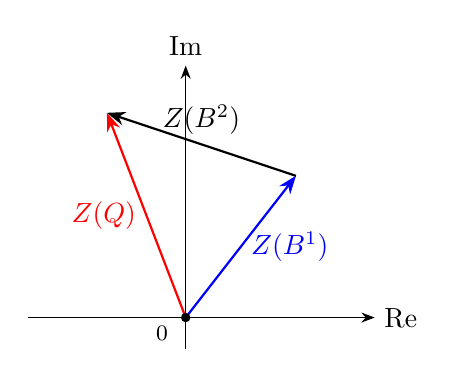
\begin{tikzpicture}[scale=2, >=Stealth]

		% 原点を中心に設定
		\coordinate (O) at (0,0);

		% 各ベクトルの終点
		\coordinate (B1) at (0.7,0.9);     % Z(A)
		\coordinate (B2) at (-1.2,0.4);    % Z(E/A)
		\coordinate (Q) at ($(B1)+(B2)$); % Z(E) = Z(A) + Z(E/A)

		% 軸
		\draw[->] (-1,0) -- (1.2,0) node[right] {\(\Re\)};
		\draw[->] (0,-0.2) -- (0,1.6) node[above] {\(\Im\)};

		\draw[->, thick,blue] (O) -- (B1) node[midway, right] {\(Z(B^1)\)};

		\draw[->, thick] (B1) -- (Q) node[midway,above] {\(Z(B^2)\)};

		\draw[->, thick,red] (O) -- (Q) node[midway, left] {\(Z(Q)\)};

		% 原点
		\fill (O) circle (0.03);
		\node at (-0.15, -0.1) {\footnotesize 0};

	\end{tikzpicture}
\end{center}
から$\phi(B^2)\ge\phi(Q)$が得られる.$\phi(B^2)=\phi(Q)=\phi(B^1)$と仮定すると,$E\twoheadrightarrow B^1$がmdqであることから$E\twoheadrightarrow B^1\twoheadrightarrow Q$となって,$B^1$と$Q$の双方向に全射があることから$B^1\simeq Q$となり,$B^2=0$.これは矛盾.したがって,$\phi(B^2)>\phi(B^1)$が成り立つ.この操作は条件(ii)より有限回でとまり,その商は半安定なのでHNフィルトレーションを得る.
\end{proof}

\begin{defn}
	$\D\colon$三角圏.$\D$上の安定性条件とは,$\D$の有界な$t$-構造のHeart $\A\subset\D$と$\A$と$\A$上の安定性条件
	\[Z\colon K(\D)=K(\A)\to\CC\]
	$(Z,\A)$のことである.
\end{defn}

\begin{defn}
	三角圏$\D$におけるスライスとは部分圏の族$\{\P(\phi)\}_{\phi\in\RR}\subset\D$で次の条件を満たすもの\\
	\bullet $\forall\phi\in\RR, \P(\phi + 1) = \P(\phi)[1]$\\
	\bullet $\phi_1>\phi_2$で$E_i\in\P(\phi_i)$ならば$\Hom_{\D}(E_1,E_2)=0$\\
	\bullet 任意の対象$E\in\D$に対して,実数列$\phi_1>\phi_2>\cdots >\phi_n$と
	\[
		\begin{tikzcd}[column sep=1.3em]
			0\ar[r,equal]&E_0\ar[rr]& & E_{1}\ar[r]\ar[ld] &\cdots\ar[r] &E_{n-2}\ar[rr]&&E_{n-1}\ar[ld]\ar[rr]&&E_n\ar[ld]\ar[r,equal]&E\\
									 &&F_{1}\ar[lu,dotted,"{[1]}"] &&&&F_{n-1}\ar[lu,dotted,"{[1]}"]&&F_n\ar[lu,dotted,"{[1]}"]
		\end{tikzcd}
	\]
	$F_i\in\P(\phi_i)$
\end{defn}

\begin{lemm}
		$\D$に安定性条件($\D$上の有界なt-構造とstability函数$Z$)をあたえることと,$\D$上のスライス$\P$と群準同型$Z\colon K(\D)\to\CC$の組$(Z,\P)$で,任意の$\phi\in\RR$と$0\neq E\in\P(\phi)$に対して$Z(E)\in\RR_{>0}e^{i\pi\phi}$を与えることは同値.
\end{lemm}

	\begin{pf}
		安定性条件$(Z,\A)\rightarrow$スライス$\P$の構成\\
		各$0<\phi\le 1$に対して,
		\[\P(\phi)\coloneq \{E\in\A\mid E\colon Z\text{-半安定 }Z(E)\in\RR_{>0}e^{i\pi\phi}\}\cup \{0\}\]
		$\phi\in\RR,\phi\in(k,k+1]$となる整数$k$をとって
		\[\P(\phi)\coloneq \P(\phi - k)[k]\]
		こう定めたとき,スライスになっていることを確かめる.\\
		\bullet $\forall\phi\in\RR, \P(\phi + 1) = \P(\phi)[1]$は定義から従う.\\
		\bullet $\phi_1 > \phi_2$と$E_i\in\P(\phi_i)$対して,$\Hom_{\D}(E_1,E_2)=0$\\
		このとき$F_1,F_2\in\P((0,1])$を用いて,$E_1=F_1[m],\ E_2=F_2[n], (m>n \text{または}\ m=n, \phi(F_1) > \phi(F_2))$とかける.\\
		$m=n$のときは補題より$0$であることがわかる.$m>n$のとき
		$\Hom_{\D}(F_1[m],F_2[n])\simeq \Hom_{\D}(F_1,F_2[-(m-n)])$なので,$\Hom_{\D}(F_1,F_2[-k])=0\ k>0$を示せばよいが,$F_1\in\D^{\le 0},\ F_2[-k]\in\D^{\ge k}$なのでt-構造の定義より$0$となることがわかる.\\
分解をもつことはt-構造の性質より,整数の列
			\[k_1>k_2 \cdots > k_n\]
			と分解
	\[
		\begin{tikzcd}[column sep=1.0em]
			0\ar[r,equal]&E_0\ar[rr]& & E_{1}\ar[r]\ar[ld] &\cdots\ar[r] &E_{n-2}\ar[rr]&&E_{n-1}\ar[ld]\ar[rr]&&E_n\ar[ld]\ar[r,equal]&E\\
									 &&A_{1}[k_1]\ar[lu,dotted,"{[1]}"] &&&&A_{n-1}[k_{n-1}]\ar[lu,dotted,"{[1]}"]&&A_n[k_n]\ar[lu,dotted,"{[1]}"]
		\end{tikzcd}
	\]
	$A_j\in \A$が存在する.各$A_j$には仮定よりHNフィルトレーションが存在するので更に分解することで3つ目の条件が得られる.\\
	逆に$\P$が与えられたとき,$\F^{\perp}[1]=\D^{\ge 0}\coloneq\P((0,\infty)), \F=\D^{\le 0}\coloneq\P((-\infty,1])$がt-構造を定める.スライスの条件より,

\end{pf}

\section{安定性条件の空間}
\begin{defn}
$\mathrm{Slice(\D)}$を$\D$上のスライスの集合,$\mathcal P,\mathcal Q\in\mathrm{Slice} \D$に対して,
\[d(\mathcal P,\mathcal Q)\coloneq\sup_{0\neq E\in\D}\{|\phi^-_{\P}(E)-\phi_{\Q}^-(E)|,|\phi^+_{\P}(E)-\phi_{\Q}^+(E)|\}\]
と定義する.距離空間の公理を満たす.
\end{defn}
\begin{lemm}
	$\phi_{*}^+(E),\phi_{*}^-(E)\colon \mathrm{Slice(\D)}\rightarrow\RR$
	は連続写像である.
\end{lemm}

\begin{thebibliography}{99}
	\bibitem{Bstab}
	Bridgeland, Tom,
		\textit{Stability conditions on triangulated categories},
	Annals of Mathematics, Vol. 166, No. 2, 2007, pp. 317–345.

	\bibitem{BBD}
	A. A. Beilinson, J. Bernstein, and P. Deligne,
	\textit{Faisceaux pervers},
	Astérisque, \textbf{100}, Société Mathématique de France, 1982. Chapitre 1.
\end{thebibliography}
\end{document}
